\documentclass{article}
\usepackage[utf8x]{inputenc}
\usepackage{ucs}
\usepackage{amsmath} 
\usepackage{amsfonts}
\usepackage{upgreek}
\usepackage[english,russian]{babel}
\usepackage{graphicx}
\usepackage{float}
\usepackage{textcomp}
\usepackage{hyperref}
\usepackage{geometry}
  \geometry{left=2cm}
  \geometry{right=1.5cm}
  \geometry{top=1cm}
  \geometry{bottom=2cm}
\usepackage{tikz}
\usepackage{ccaption}
\usepackage{multicol}
%\setlength{\columnsep}{1.5cm}
%\setlength{\columnseprule}{0.2pt}
\usepackage{listings}

\begin{document}
\pagenumbering{gobble}

\lstset{
  language=C,                % choose the language of the code
  basicstyle=\linespread{1.1}\ttfamily,
  columns=fixed,
  fontadjust=true,
  basewidth=0.5em,
  keywordstyle=\color{blue}\bfseries,
  commentstyle=\color{gray},
  stringstyle=\ttfamily\color{orange!50!black},
  showstringspaces=false,
  %numbers=false,                   % where to put the line-numbers
  numbersep=5pt,
  numberstyle=\tiny\color{black},
  numberfirstline=true,
  stepnumber=1,                   % the step between two line-numbers.        
  numbersep=10pt,                  % how far the line-numbers are from the code
  backgroundcolor=\color{white},  % choose the background color. You must add \usepackage{color}
  showstringspaces=false,         % underline spaces within strings
  captionpos=b,                   % sets the caption-position to bottom
  breaklines=true,                % sets automatic line breaking
  breakatwhitespace=true,         % sets if automatic breaks should only happen at whitespace
  xleftmargin=.2in,
  extendedchars=\true,
  keepspaces = true,
}
\lstset{literate=%
   *{0}{{{\color{red!20!violet}0}}}1
    {1}{{{\color{red!20!violet}1}}}1
    {2}{{{\color{red!20!violet}2}}}1
    {3}{{{\color{red!20!violet}3}}}1
    {4}{{{\color{red!20!violet}4}}}1
    {5}{{{\color{red!20!violet}5}}}1
    {6}{{{\color{red!20!violet}6}}}1
    {7}{{{\color{red!20!violet}7}}}1
    {8}{{{\color{red!20!violet}8}}}1
    {9}{{{\color{red!20!violet}9}}}1
}


\title{Семинар \#11: Связный список. Домашнее задание.\vspace{-5ex}}\date{}\maketitle
На классном занятии был пройден односвязный список. Он имеет несколько преемущевств по сравнению с массивом, например, быстрая вставка элементов в начало и быстрое удаление из начала. Однако у него есть также ряд недостатков. К примеру, чтобы удалить элемент из конца односвязного списка, нужно пройти по всему списку, чтобы найти указатель на предпоследний узел, а это долго ($O(N)$). Аналогичная проблема есть и при вставке/удалении в середину списка. Эти проблемы решаются в двусвязном списке. В таком списке в каждом узле хранится не только указатель на следующий элемент, но и указатель на предыдущий. Также, помимо указателя на начало списка(\texttt{head}) будем отдельно хранить указатель на конец списка(\texttt{tail}). В результате все операции по вставке и удалению будут занимать $O(1)$.\\

Связный список используется там где нужно хранить набор элементов, в который нужно часто добавлять и удалять элементы.
Также связный список используется как составная часть других структур данных (хештаблицы, графы и др.).
\begin{center}
\begin{tabular}{ c c c c }
 Операция & Массив & Односвязный список & Двусвязный список\\ 
 \hline
 Доступ по номеру & $O(1)$ & $O(N)$ & $O(N)$  \\
 Поиск & $O(N)$ & $O(N)$ & $O(N)$  \\    
 Вставка в начало & $O(N)$ & $O(1)$ & $O(1)$  \\
 Вставка в конец & $O(1)$ & $O(N)$ & $O(1)$  \\
 Вставка в середину (по указателю на элемент) & $O(N)$ & $O(1)$ после и $O(N)$ до элемента & $O(1)$  \\
 Удаление из начала & $O(N)$ & $O(1)$ & $O(1)$  \\
 Удаление из конца & $O(1)$ & $O(N)$ & $O(1)$  \\
 Удаление из середины (по указателю на элемент) & $O(N)$ & $O(N)$ & $O(1)$  \\
\end{tabular}
\end{center}

Для реализации двусвязного списка на языке \texttt{C} дополнительно к структуре \texttt{Node} создадим структуру \texttt{List}, которая будет хранить 2 указателя \texttt{head} и \texttt{tail}.

\begin{center}
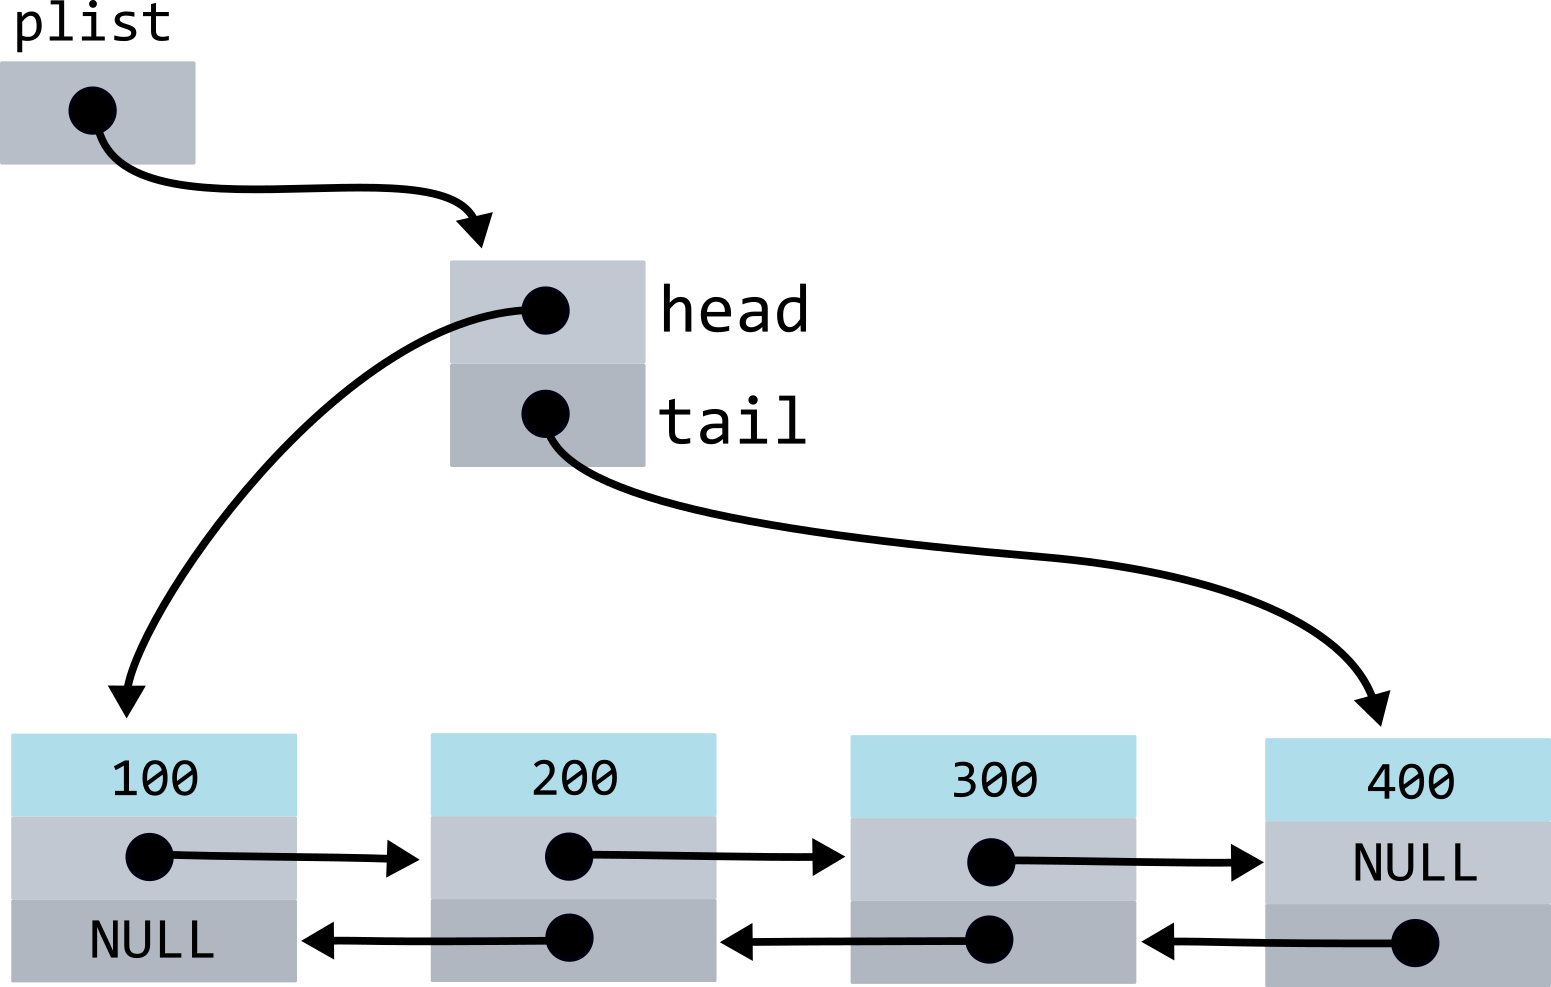
\includegraphics[scale=1]{../images/doublylist/doublylist_overview.png}
\end{center}

\newpage
\subsection*{Задачи}
Начальный код в файле \texttt{doublylist.c}. В этом файле уже написаны следующие функции:
\begin{itemize}
\item \texttt{List* list\_create()} -- инициализирует список (создаёт и возвращает список нулевого размера). Эта функция выделяет память под структуру \texttt{List}, задаёт \texttt{head} и \texttt{tail} и возвращает указатель на эту структуру.
\item \texttt{void list\_print(const List* plist)} -- распечатывает все элементы списка.
\item \texttt{void list\_add\_last(List* plist, int x)} -- добавляет элемент \texttt{x} в конец списка.
\end{itemize}
Напишите следующие функции для работы с двусвязным списком:
\begin{enumerate}
\item \texttt{int list\_size(const List* plist)} -- возвращает количество элементов списка.
\item \texttt{void list\_add\_first(List* plist, int x)} -- добавляет элемент \texttt{x} в начало списка. Отдельно рассмотрите случай, когда список пуст.
\item \texttt{void list\_insert\_after(List* plist, Node* p, int x)} -- добавляет элемент \texttt{x} сразу после узла, на который указывает \texttt{p}. Нужно рассмотреть несколько случаев:
\begin{enumerate}
\item Когда список пуст
\item Когда \texttt{p} указывает на последний элемент
\item Остальное
\end{enumerate}
\item \texttt{int list\_remove\_first(List* plist)} -- удаляет элемент из начала списка и возвращает его значение. Не забудьте изменить \texttt{head}. Отдельно рассмотрите случаи когда список пуст и когда он состоит из одного элемента.
\item \texttt{int list\_remove\_last(List* plist)} -- удаляет элемент из конца списка и возвращает его значение. Не забудьте изменить \texttt{tail}. Отдельно рассмотрите случаи когда список пуст и когда он состоит из одного элемента.
\item \texttt{int list\_remove(List* plist, Node* p)} -- удаляет элемент на который указывает \texttt{p} и возвращает его значение. Нужно рассмотреть несколько случаев:
\begin{enumerate}
\item Когда список пуст. Нужно написать сообщении об ошибке и выйти(\texttt{exit(1)}).
\item Когда список состоит из одного элемента.
\item Когда элементов больше 1, а \texttt{p} указывает на первый элемент.
\item Когда элементов больше 1, а \texttt{p} указывает на последний элемент.
\item Остальное
\end{enumerate}

\item \texttt{Node* list\_find(const List* plist, int x)} -- ищет элемент \texttt{x} в связном списке и возвращает указатель на соответствующий узел. Если такого элемента нет, то функция должне вернуть \texttt{NULL}.
\item \texttt{int list\_destroy(List* plist)} -- освобождает всю память, выделенную под список. Так как память выделялась под каждый элемент отдельно, то освобождать нужно также каждый элемент по отдельности. Также нужно не забыть освободить структуру \texttt{List}.

\item Реализовать абстрактный тип данных стек(Queue) на основе двусвязного списка.

\item В этой задаче вам нужно будет создать заголовочные файлы (другое название \texttt{header}-файлы). Это файлы с расширением \texttt{.h}, которые содержат код и подключаются к программе с помощью директивы \texttt{\#include}. Директива \texttt{\#include} ищет файл(в текущей директории или в специальных системных папках) и просто вставляет всё содержимое этого файла на место директивы.\\

Создать \texttt{header}-файлы \texttt{doublylist.h} и \texttt{queue.h} (если сделали предыдущую задачу), в которых будет храниться реализация двусвязного списка и очереди. Создайте новую программу \texttt{main.c}, в которой протестируйте ваши реализации, включив заголовочные файлы \texttt{doublylist.h} и \texttt{queue.h}. Чтобы избежать многократного включения \texttt{header}-файлов используйте директиву \\
\texttt{\#pragma once}\\

В качестве примера можете посмотреть решения классных задач \texttt{list.h} и \texttt{stack.h}.
\end{enumerate}

\end{document}